\documentclass[../main.tex]{subfiles}
\begin{document}

\subsection{Probenpräperation mit Polarisationspulsen}

    Das Erdmagnetfeld $\vec B_0$ ist vergleichsweise schwach und würde eine für genaue Messungen zu kleine Magnetisierung der Probe liefern. Deshalb wird zuerst immer ein Polarisationspuls $\vec B_0$ ausgesandt, welcher durch induzierte Spintransitionen eine größere Magnetisierung $\vec M$ bewirkt. Beim Herunterfahren des Polarisationspulses ist zweierlei zu beachten:
    \begin{itemize}
        \item Sie muss schnell genug geschehen, damit $\vec M$ nicht währenddessen verschwindet.
        \item Sie muss aber auch adiabatisch verlaufen, d.h. langsam genug, damit die Ausrichtung von $\vec M$ der Gesamtrichtung des externen Feldes folgt. Am Anfang zeigt $\vec M$ also fast vollständig in Richtung $\vec B_p$, am Ende idealerweise in Richtung $\vec B_0$ \cite[p.19]{doc:EFNMRStudentManual}. % wieso erreicht ein langsameres Herunterfahren dies?
    \end{itemize}

\subsection{Longitudinale Spin-Gitter-Relaxion}
    In diesem und im folgenden Abschnitt \textit{bezeichne die $z$-Achse, auch longitudinale Achse genannt, jene Achse parallel zum dominanten externen Magnetfeld}. Die Spin-Gitter-Relaxtion bezeichnet die Relaxion der $z$-Magnetisierung eines Spin-Ensambles hinzu des Gleichgewichtszustandes. Dies geschieht durch Interaktion mit dem lokalen $\vec{B}_{loc}$-Feld. Dessen $x-y$-Komponenten präzidieren ebenfalls nahe der Larmorfrequenz und können deshalb Transitionen der Spinzustände induzieren \cite[p.2]{PhysRev.110.65}. Letztlich führt dies zu einer Erhöhung oder eines Abbaus der Magnetisierung $M_z$, beschrieben durch:
    \[
        M_z(t) = \frac{M_0 - M_z(t)}{T_1}.
    \]
    $T_1$ ist die charakteristische Relaxionszeit und $M_0$ die Gleichgewichtsmagnetisierung. Im Polarisationsfeld $\vec{B}_p$ mit $M_z(0)\approx 0$ ergibt sich die Lösung \cite[p.35]{doc:EFNMRStudentManual}
    \[
        M_z(t) \approx M_p\cdot\nbra{1 - \exp(-\frac{t}{T_1})}
    \]
    und im reinen Erdmagnetfeld $\vec{B}_e\approx 0$ anschließend
     \[
        M_z(t) \approx M_p\cdot\exp(-\frac{t}{T_1}).
    \]

\subsection{Transversale Spin-Spin-Relaxion}
    Transversale Relaxion bezeichnet das Verschwinden der $M_x,M_y$-Komponenten, während $M_z$ den Gleichgezwichtszustand anstrebt. Der Grund für die Relaxion ist, dass die Spins eines Ensembles aufhören in Phase zu präzidieren und somit das magnetische Gesamtmoment reduzieren. Je nach genauen Prozess wird Energie oder keine Energie übertragen. Es gibt zwei grobe Kategorien der Wechselwirkung:
    \begin{itemize}
        \item Zum einen tragen auch die $x-y$-Komponenten des lokalen Felds $\vec{B}_{loc}$ dazu bei - diese präzidieren alle mit kleinen Frequenzschwankungen $\Delta\omega$. Da diese den zufälligen Bewegungen der Moleküle in der Umgebung unterliegen, ist diese Relaxion irreversibel.
        \item Hinzu kommt aber auch die Wechselwirkung mit der $z$-Komponente von $\vec{B}_loc$. Dieser präzidiert zwar nicht mit der Larmorfrequenz, liefert aber zum $\vec{B}_0$-Feld eine Inhomogenität $\Delta B_0$, was zu einem breiteren Energiespektrum führt \cite[p.2]{PhysRev.110.65}.
    \end{itemize}
    Die Magnetisierung $M_{x,y}$ folgt einem exponentiellen Zerfall
    \[
        M_{x,y}(t) = M_{x,y,0}\cdot\exp(-\frac{t}{T_2^*}),
    \]
    mit einer charakteristischen Zerfallszeit
    \begin{align*}
        \frac{1}{T_2^*} = \frac{1}{T_2} + \gamma\cdot\Delta B_0.
    \end{align*}
    $T_2$ bezieht sich auf den irreversiblen Anteil der Relaxion \cite[p.41]{doc:EFNMRStudentManual}.

\subsection{Mehrdimensionales MRI}
    MRI (\textit{Magnetic Resonance Imaging}) beruht darauf, dass durch ein linear variierendes Magnetfeld $\vec B_{exp}$ die Larmorfrequenzs von Kernspins dessen Position enkodiert. Im zweidimensionalen Fall ergibt sich:
    \begin{align*}
        \vec B_{ex} &= (G_y\cdot y)\cdot\vec e_y + (G_z\cdot z)\cdot\vec e_z\\
        \omega(y, z) &= \gamma\cdot\nbra{G_y\cdot y + G_z\cdot z}
    \end{align*}
    Ohne Einschränkung der Allgemeinheit wurde hier angenommen, dass $\vec B_{ex}$ keine statistische Komponente besitzt, da eine solche durch Kalibrierung herausgefiltert werden kann. Bei einer Kernspindichte von $\rho$ ist das in diesem Fall messbare Signal eines gesamten y-z-Auschnitts der Probe: 
    \begin{align*}
        S(t) &= \int_{\R^2} \rho(y,z)\cdot\exp(-\cmath\gamma\cdot\omega(x,y)\cdot t)\,d(y,z)\\
        &= \int_{\R^2}\rho(y,z)\cdot\exp(-2\pi\cmath\cdot\scpr{\vec{k}(\vec{G}, t)}{\vec{r}})\, d\vec{r} =: \tilde S(k(\vec{G}, t)),
    \end{align*}
    mit der Definition 
    \begin{align}
        k(\vec{G}, t):= \frac{1}{2\pi}\cdot \gamma\cdot\vec{G}.
        \label{eq:GrundlagenMehrdimMRIkVektor}\cdot t
    \end{align}
    Eine anschauliche Erklärung von $k(\vec{G}, t)$ als Wellenvektor ist folgende: durch das lineare variierene Magneteld beginnen auch die Kernspins einer mit der Zeit und dem Ort lineare Phasendifferenz aufzubauen:
    \[ 
        \Delta\Phi(\vec{G}, x,y,t) = \omega\cdot t = \gamma\cdot(G_y\cdot y + G_z\cdot z)\cdot t = 2\pi\cdot \scpr{k(\vec{G},t)}{\vec r}.
    \]
    Dadurch erzeugen die Spitzen der Kernspins eine Helixstruktur, deren Periodizität gerade durch $\lambda = 2\pi/ k(\Vec{G},t)$ gegeben ist.\\

    Eine inverse Fouriertransformation von $\tilde S$ liefert nun die gewünschten Rauminformationen:
    \[
        \rho(y,z) = (\mathcal{F}^{-1}\tilde S)(y,z) = \int_{\R^2} \tilde S(k)\cdot\exp(\cmath 2\pi\cdot\scpr{\vec{k}}{\vec {r}})\,d\vec{k}.
    \]
    Dieser Ausdruck lässt sich mit dem Zeitsignal $S(t)$ und Zusammenhang \eqref{eq:GrundlagenMehrdimMRIkVektor} berechnen \cite[p.61-63]{doc:EFNMRStudentManual}.\\

    Um den gewünschten zweidimensionalen $\vec{k}$-Raum mit einem eindimensionalen positiven Zeitparameter abrastern zu können, werden zwei Möglichkeiten vorgestellt:
    \begin{itemize}
        \item \textbf{Gradient-Echo-Imaging}. Es werden ein Polarisationspuls und ein $\pi/2$-Puls ausgesandt (1). Anschließend werden (2) ein $G_y$- und ein $G_z$-Gradientenfeld angelegt für eine gewisse Zeit $t_{Grad}$, bis ein gewisses $\vec{k}_{min}(\vec{G}, t_{Grad})$ erreicht wird (3). Danach wird z.B. $G_y$ deaktiviert und $G_z$ invertiert, sodass \textit{$\vec{k}$ sich genau in die entgegengesetzte z-Richtung entwickelt}. Wird ein gewünschtes $\vec{k}_{\max}(\vec{G}', t_{End})$ erreicht, so ist die Messung beendet.\\

        Zusammengefasst: $G_y$ sorgt für die Auswahl einer $k_z$-Linie, welche durch cleveres Schalten von $G_z$ von $k_{z,\min}<0$ bis $k_{z,max}>0$ abgerastert wird. Abbildung \ref{fig:GrundlagenMehrdimMRIGradientecho} verdeutlicht dies schematisch \cite[p.74]{doc:EFNMRStudentManual}.

        \begin{figure}[H]
            \centering
            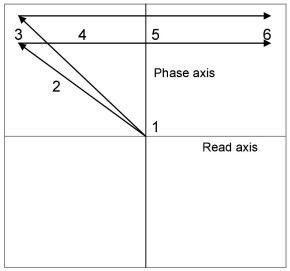
\includegraphics[width=0.4\textwidth]{Bilddateien/GrundlagenMehrdimMRIGradientecho.jpg}
            \caption{Trajektorie im $\vec{k}$-Raum für unterschiedlich starke y-Gradienten $G_y$. \textit{Phase axis} ist hier die $y$-Achse und \textit{Read axis} die $z$-Achse \cite[p.74]{doc:EFNMRStudentManual}.}
            \label{fig:GrundlagenMehrdimMRIGradientecho}
        \end{figure}
        
        \item \textbf{Spin-Echo-Imaging}. Wieder werden ein Polarisationspuls und ein $\pi/2$-Puls ausgesandt (1). Anschließend werden aber drei Gradientenfelder eingeschalten, z.B. ein Read-Gradient $G_z$ und zwei Phasengradienten $G_{y,1}, G_{y,2}$. Wird ein gewisses $\vec{k}_{min, flipped}(\vec{G}, t)$ erreicht, fahren $G_{y,2}, G_{y,2}$ herunter, $G_z$ bleibt bestehen (2). \textit{Die Umkehrung der Laufrichtung wird nun durch einen $\pi$-Puls erreicht (3)}. Dabei wird der $\vec k$-Vektor hinzu 
        \[
        \vec{k}_{min}(\vec{G}, t) = -\vec{k}_{min, flipped}(\vec{G}, t).
        \]
        gespiegelt. Das $G_z$-Feld sorgt nun für ein Abrastern entlang der selektierten $z$-Linie \cite[p.81-82]{doc:EFNMRStudentManual}. Schema \ref{fig:GrundlagenMehrdimMRISpinecho} verdeutlicht dies.

        \begin{figure}[H]
            \centering
            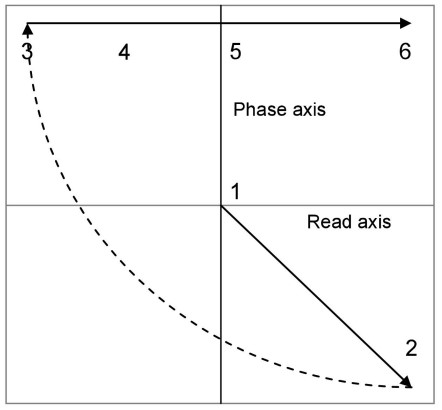
\includegraphics[width=0.4\textwidth]{Bilddateien/GrundlagenMehrdimMRISpinecho.jpg}
            \caption{Trajektorie im $\vec{k}$-Raum durch ein Spin-Echo. \textit{Phase axis} ist hier die $y$-Achse und \textit{Read axis} die $z$-Achse \cite[p.82]{doc:EFNMRStudentManual}.}
            \label{fig:GrundlagenMehrdimMRISpinecho}
        \end{figure}
    \end{itemize}

\end{document}